\chapter{Version Control}
	Door middel van version control kunnen meerdere ontwikkelaars aan dezelfde software werken.
	Tijdens het project zal Git (GitHub) gebruikt worden voor version control. Er is hiervoor gekozen omdat hiermee reeds de meeste ervaring is opgedaan.
	
	\begin{figure}[H]
			\includegraphics[width=0.50\textwidth]{images/configuredBranches.png}
			\caption{Overzicht van default branch en protected branches}
			\label{fig:ConfiguredBranches}
	\end{figure}
	
	\section{Branches}
	Voor de repository waar de code van de verschillende applicaties wordt bijgehouden, zijn verschillende branches aangemaakt. Wat het nu is van deze verschillende branches, staat in de volgende alinea's uitgelegd.
	
	\begin{figure}[H]
			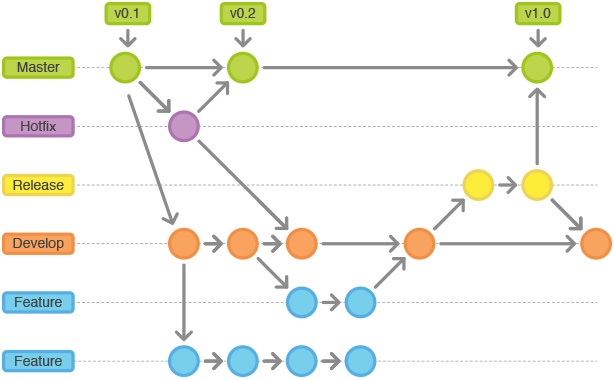
\includegraphics[width=0.75\textwidth]{images/BranchScheme.png}
			\caption{Schematisch overzicht van de branches}
			\label{fig:BranchScheme}
	\end{figure}
	
	\subsection{Master}
	De code die beschikbaar is in de master-branch, is de code van de software versie die in productie gebruikt wordt. Nieuwe functies of bug fixes mogen dan ook niet rechtstreeks naar deze branch gecommit worden.
	Deze branch is tevens protected. Dit wilt zeggen dat vanuit een git programma (UI of CLI) niet rechtstreeks naar deze branch gecommit kan worden. Dit zorgt ervoor dat een ontwikkelaar niet per ongeluk naar deze branch kan committen.
	
	
	\begin{figure}[H]
	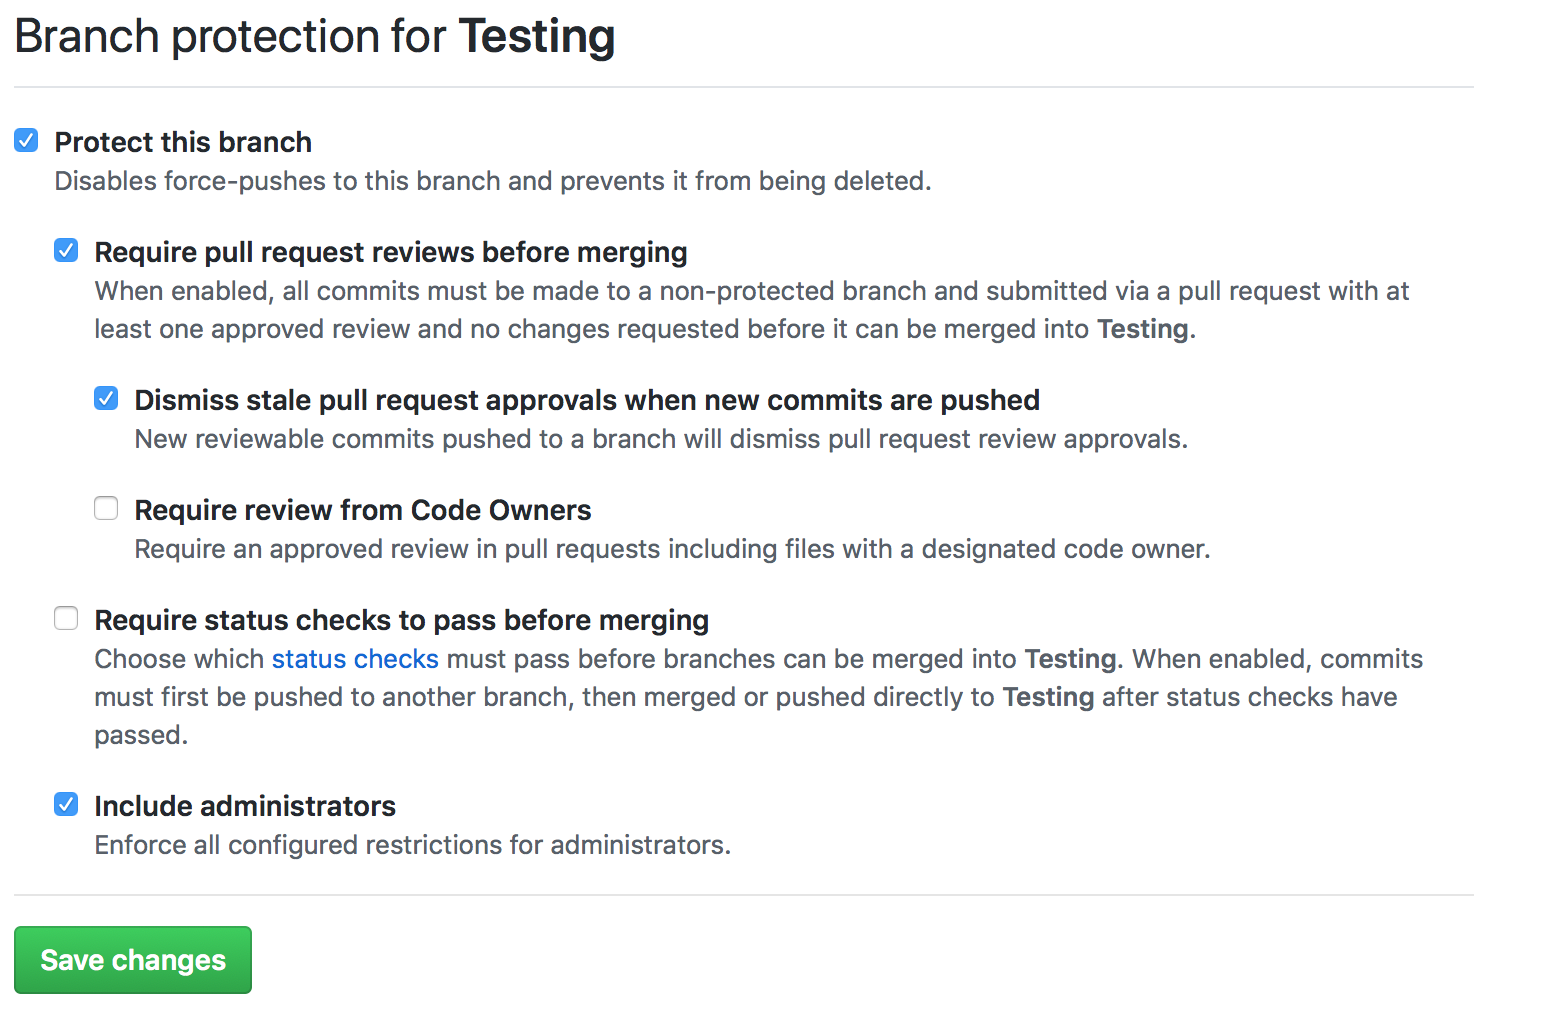
\includegraphics[width=0.5\textwidth]{images/BranchProtectionSetup.png}
	\caption{Overzicht van protectie wat ingesteld is op branch}
	\label{fig:BranchProtectionSetup}
	\end{figure}

	\subsection{Hotfix}
	Wanneer een probleem ontdekt is op de productie omgeving wat een grote impact heeft op de werking van de applicatie(s), dan moet dit natuurlijk zo snel mogelijk opgelost worden. 
	
	Om de urgentie van een probleem in de productie omgeving te bepalen, zal dit overlegd worden met de SCRUM master, Product Owner en de klant. Wanneer de urgentie dermate hoog is dat het probleem zo snel mogelijk moet worden opgelost, kan dit gedaan worden aan de hand van een hotfix.
	Wanneer er besloten is om het probleem door middel van een hotfix op te lossen, zal de SCRUM master in de backlog een nieuw issue aanmaken.
	
	De hotfix zal geïmplementeerd worden door gebruik te maken van de huidige code in de productie omgeving. De ontwikkelaar maakt dus een nieuwe branch aan vanuit de master omgeving. De benaming van de branch bevat altijd de prefix "hotfix-", gevolgd door het nummer van de issue in de backlog. Op deze manier is het meteen voor iedereen duidelijk welk issue opgelost gaat worden in de nieuwe branch.
	
	Wanneer het probleem opgelost en getest is, kan de nieuwe code na akkoord van de release manager toegevoegd worden aan de productie omgeving.
	
	Naast de Testing branch, is een hotfix branch de enige manier om rechtstreeks nieuwe code toe te voegen aan de master branch.
	
	\subsection{Testing}
	De Testing-branch zal gebruikt worden om nieuwe functionaliteit die ontwikkeld zijn in de development branch te testen. Wanneer de functionaliteit in de testing branch geaccepteerd wordt, zal deze worden doorgezet naar de master branch zodat de verbeteringen en/of nieuwe wijzigingen beschikbaar zijn voor alle gebruikers op de productie omgeving.
	De Testing-branch heeft dezelfde setup als de Master-branch. Dit wilt zeggen dat het op deze branch ook niet mogelijk is om rechtstreeks code te committen.
	
	De testing omgeving die gebruikt wordt om de code van de testing branch beschikbaar te stellen, kan tevens gebruikt worden door testers om nieuwe functionaliteit of verbeteringen te testen. Daarnaast kan de release manager akkoord geven op de versie die in deze omgeving staat, waardoor deze verplaatst zal worden naar de productie omgeving.
	\subsection{Development}
	
	De Development-branch bevat nieuwe functionaliteit of verbeteringen die ontwikkeld zijn. Deze branch is vrij toegangkelijk voor de ontwikkelaar om eventueel kleine(re) verbeteringen door te voeren.	
	Het is als nog de bedoeling dat nieuwe functionaliteit niet rechtstreeks op deze branch wordt gecommit. Mocht een ontwikkelaar nieuwe functionaliteit of grotere verbeteringen willen ontwikkelen, kan hiervoor een zogenaamde Feature-branch worden aangemaakt. Meer informatie hierover is in de volgende alinea te lezen
	
	\subsection{Features}
	De Features-branch is geen branch die direct aangemaakt is op Github. Dit komt doordat "Features"\ een overkoepelende term is. Wanneer een ontwikkelaar nieuwe functionaliteit of verbeteringen wilt ontwikkelen, dan zal hiervoor een nieuwe branch moeten worden aangemaakt, bijvoorbeeld "Dev-exampleFeature". Aan de hand van de prefix "Dev-" weet iedereen dat dit een branch betreft waar nieuwe functionaliteit of verbeteringen op worden ontwikkeld. Het gedeelte achter de prefix moet dan ook beschrijven aan welke functionaliteit of verbeteringen worden gewerkt.
	
	
	Wanneer de ontwikkelaar het implementeren heeft voltooid, zal dit eerst getest moeten worden op zijn eigen, lokale omgeving. Wanneer die nieuwe functionaliteit werkt met de rest van de ontwikkelde software, kan de ontwikkelaar zijn branch, bijvoorbeeld "Dev-exampleFeature"\ gaan samenvoegen met de Development-branch. Hiervoor maakt de ontwikkelaar een merge request aan wat ervoor zorgt dat de nieuwe code wordt samengevoegd op de Development-branch.
	
	\subsection{Bugfix}
	In hoofdstuk 3.1.2 Hotfix werd beschreven dat samen met de SCRUM master, product owner en klant de urgentie van een probleem wordt bepaald.
	Wanneer ervoor gekozen wordt dat de urgentie niet hoog genoeg is om het probleem direct, door middel van een hotfix, op te lossen, zal het probleem opgelost worden door middel van een bugfix. Ook hierbij zal de SCRUM master een nieuw issue is de backlog aanmaken.
	
	De implementatie van een bugfix wordt op dezelfde manier uitgevoerd als een nieuwe feature, het verschil is enkel de benaming van de branch. In plaats van de prefix "Dev-", zal de prefix "Bugfix-" gebruikt worden gevolgd door het issue nummer zoals dit bekend is in de backlog.

	\subsection{Patch}
	Vaak wordt er bij het ontwikkelen van de applicaties verschillende libraries gebruikt die verschillende functionaliteit met zich meebrengt. Vaak worden de gebruikte libraries doorontwikkeld waardoor deze na een bepaalde tijd nieuwe functionaliteit kunnen bevatten. Op moment dat de software die door ons ontwikkeld wordt gebruik wilt maken van deze nieuwe functionaliteit, moet meestal de library worden bijgewerkt. Dit kan aan de hand van een Patch gebeuren. 
	
	Daarnaast kan het soms voorkomen dat in een library een fout zit waar omheen gewerkt moet worden, een zogenaamde "hack". Ook deze oplossingen worden geïmplementeerd aan de hand van een patch branch.
	
	Om een patch door te voeren op de software, zal een ontwikkelaar een nieuwe branch aanmaken vanuit de developement branch. Deze branch bevat de prefix "patch-" gevolgd door de naam van de library die bijgewerkt wordt of waar een hack voor wordt geïmplementeerd. Wanneer de nieuwe code is getest en in orde is bevonden door de ontwikkelaar, kan de aangemaakte patch brand weer samengevoegd worden met de development branch.